\def\mySecNum{11.3}
\mySection{\mySecNum~The Binomial tree and lognormality}
%-------------- start slide -------------------------------%{{{ 1
\begin{frame}[fragile,t]
\begin{center}

	The usefulness of the binomial pricing model hinges on \\

	\bigskip

	the binomial tree providing                            \\

	\bigskip
	a reasonable representation of                         \\

	\bigskip

	\textcolor{magenta}{the stock price distribution}
	\bigskip
	\bigskip

	\mySeparateLine
	\bigskip

	The binomial tree approximates a lognormal distribution
\end{center}

\end{frame}
%-------------- end slide -------------------------------%}}}
%-------------- start slide -------------------------------%{{{ 1
\begin{frame}[fragile,t]
	\frametitle{Random Walk}
\begin{itemize}
	\item Let $Y_i$ be a sequence of i.i.d. random variables, each following
		\begin{equation*}
			Y_i =
			\begin{cases}
				1  & \text{with probability $1/2$} \\
				-1 & \text{with probability $1/2$}
			\end{cases}
		\end{equation*}
	\item Random walk $Z_n$ is defined to be
		\begin{equation*}
			Z_n = \sum_{i=1}^{n} Y_i.
		\end{equation*}
		\bigskip
	\item From the walk $Z_n$, one can also retrieve the values of $Y_n$
		\begin{equation*}
			Y_n = Z_n - Z_{n-1}
		\end{equation*}
\end{itemize}
\end{frame}
%-------------- end slide -------------------------------%}}}
%-------------- start slide -------------------------------%{{{ 1
\begin{frame}[fragile,t]
\begin{center}
	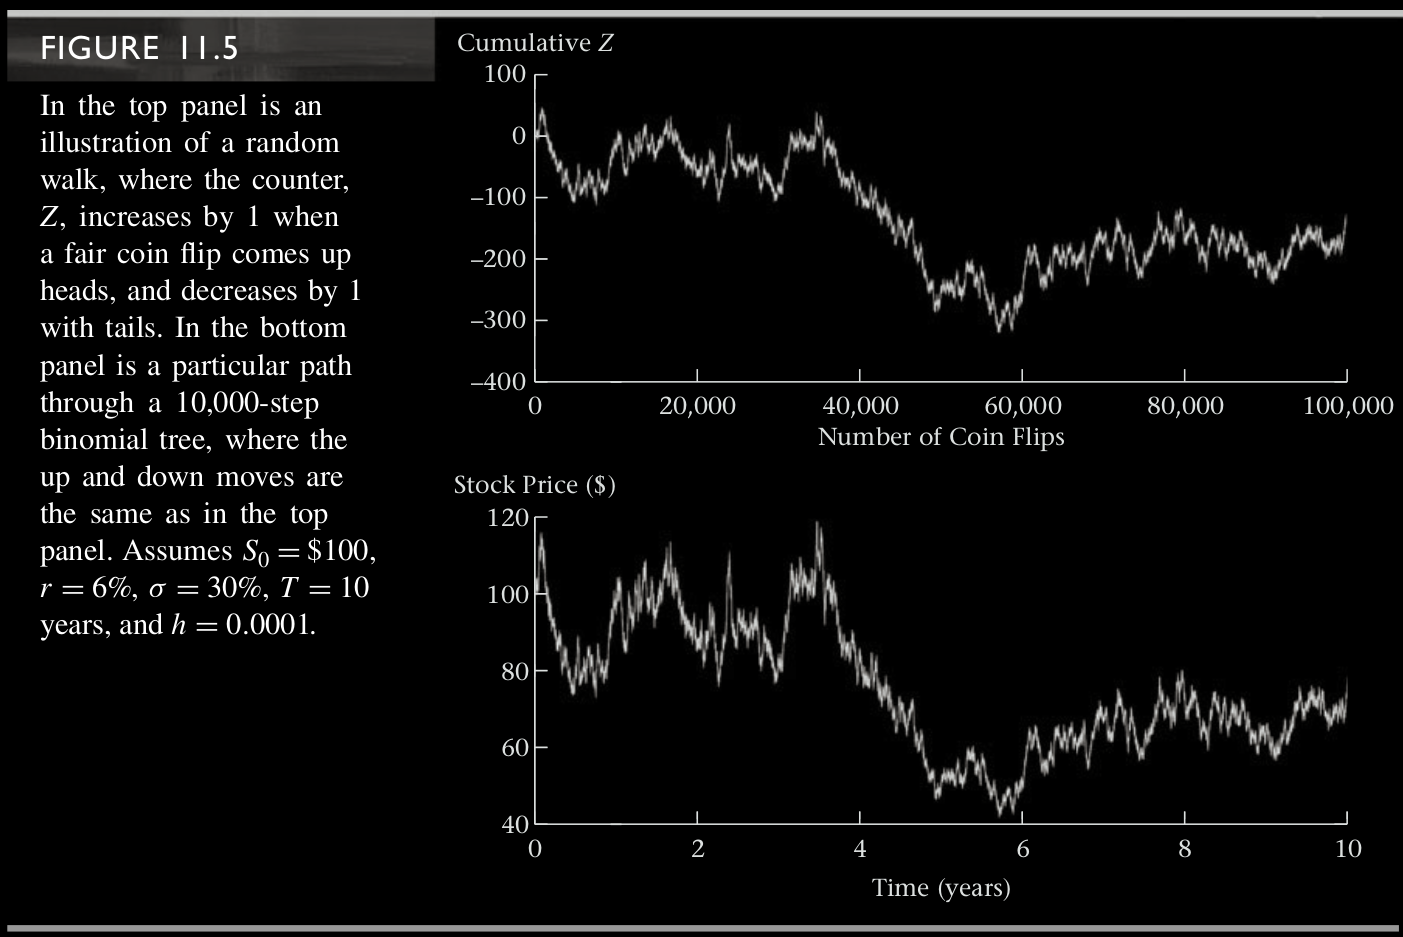
\includegraphics[scale=0.25]{figs/Figure-11-5.png}
\end{center}
\end{frame}
%-------------- end slide -------------------------------%}}}
%-------------- start slide -------------------------------%{{{ 1
\begin{frame}[fragile]
	\frametitle{Modelling Stock prices as a random walk}

	\begin{center}

		The idea that asset prices should follow a random walk was articulated in Samuelson (1965)
		\vfill

		In efficient markets, an asset price should reflect all available information. \\

		In response to new information the price is equally likely to move up or down, as with the coin
		flip.

		\vfill

		The price after a period of time is the initial price plus the cumulative up and down movements
		due to informational surprises

	\end{center}
\end{frame}
%-------------- end slide -------------------------------%}}}
%-------------- start slide -------------------------------%{{{ 1
\begin{frame}[fragile,t]
	\frametitle{Modelling Stock prices as a random walk \\ -- Issues and Binomial Model}
	\begin{center}

		If by chance we get enough cumulative down movements, the stock price will become negative
		\vfill

		The stock, on average, should have a positive return. The random walk model taken literally does not permit this
		\vfill

		The magnitude of the move (\$1) should depend upon how quickly the coin flips occur and the level of the stock price
		\vfill

		\mySeparateLine
		\bigskip

		The \textcolor{magenta}{binomial model} is a variant of the random walk model \\
		that solves all of these problems at once:
		\begin{equation*}
			S_{t+h} = S_t e^{(r-\delta)h \pm \sigma h},
		\end{equation*}
		which says, instead of the prices jumping like a random walk,\\
		the compound rate follows a random walk.
	\end{center}
\end{frame}
%-------------- end slide -------------------------------%}}}
%-------------- start slide -------------------------------%{{{ 1
\begin{frame}[fragile,t]
	\frametitle{Lognormality of the binomial model}
	\begin{center}

		The binomial tree approximates a lognormal distribution, which is commonly used to model stock
		prices
		\vfill

		The lognormal distribution is the probability distribution that arises from the assumption that
		continuously compounded returns on the stock are normally distributed
		\vfill

		With the lognormal distribution, the stock price is positive, and the distribution is skewed to the
		right, that is, there is a chance that extremely high stock prices will occur

	\end{center}
\end{frame}
%-------------- end slide -------------------------------%}}}
%-------------- start slide -------------------------------%{{{ 1
\begin{frame}[fragile,t]
\begin{center}
	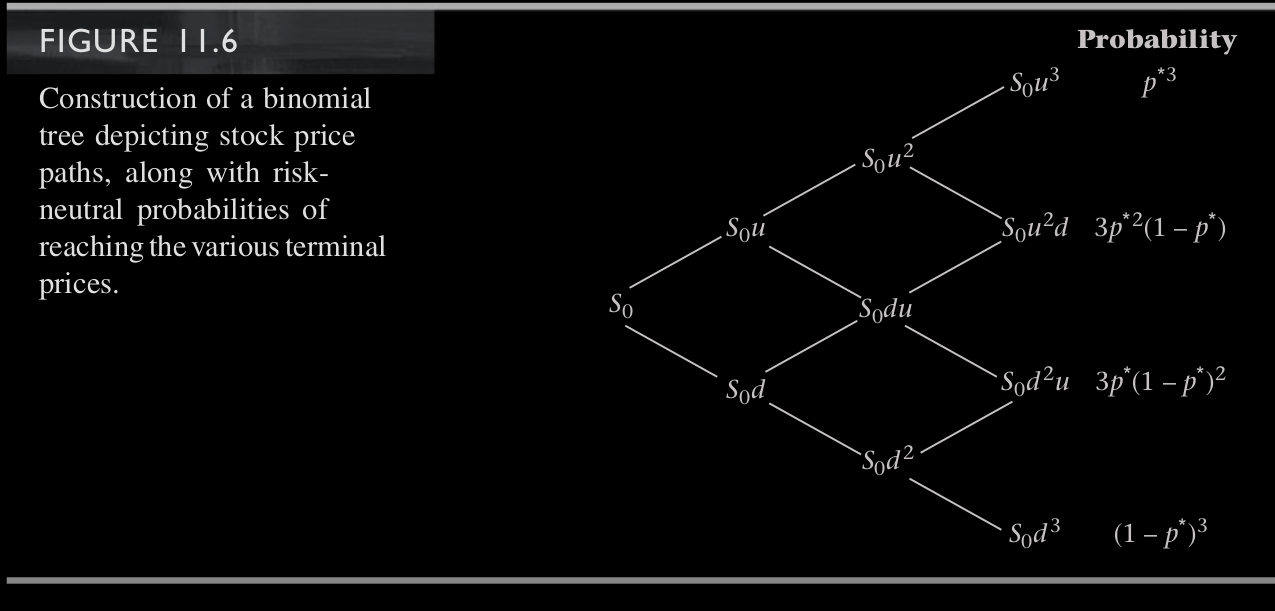
\includegraphics[scale=0.25]{figs/Figure-11-6.png}
\end{center}
\end{frame}
%-------------- end slide -------------------------------%}}}
%-------------- start slide -------------------------------%{{{ 1
\begin{frame}[fragile,t]
\begin{center}
	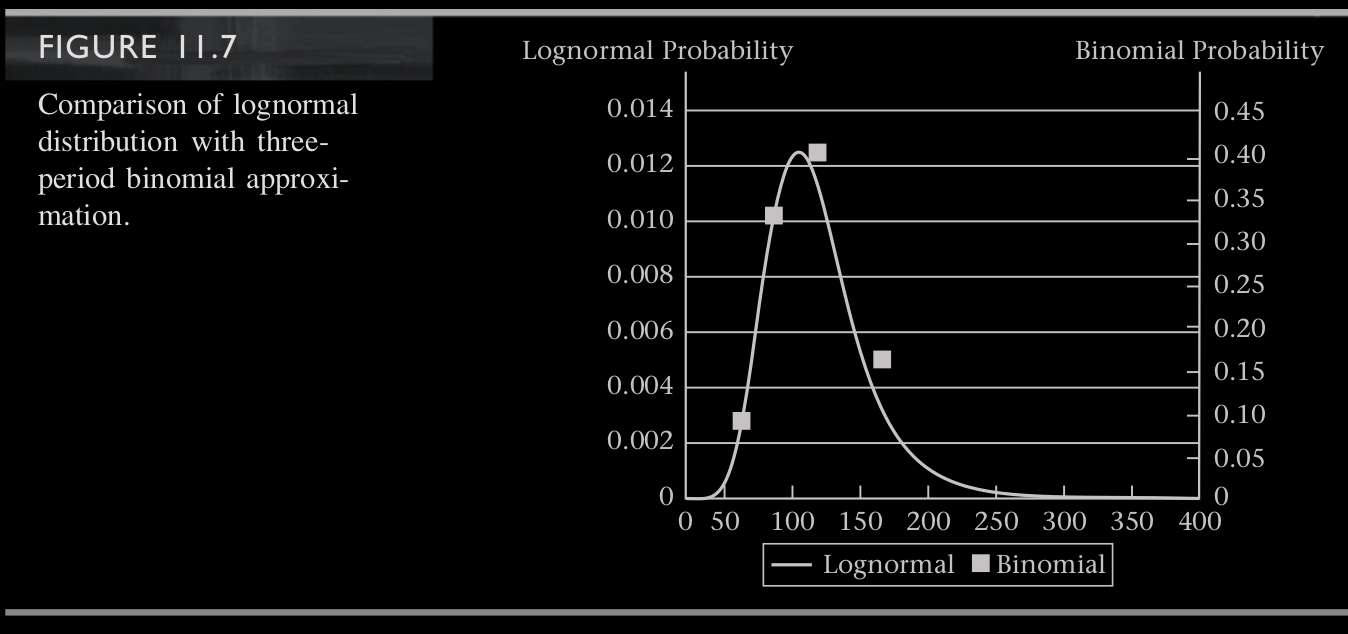
\includegraphics[scale=0.2]{figs/Figure-11-7.png}
	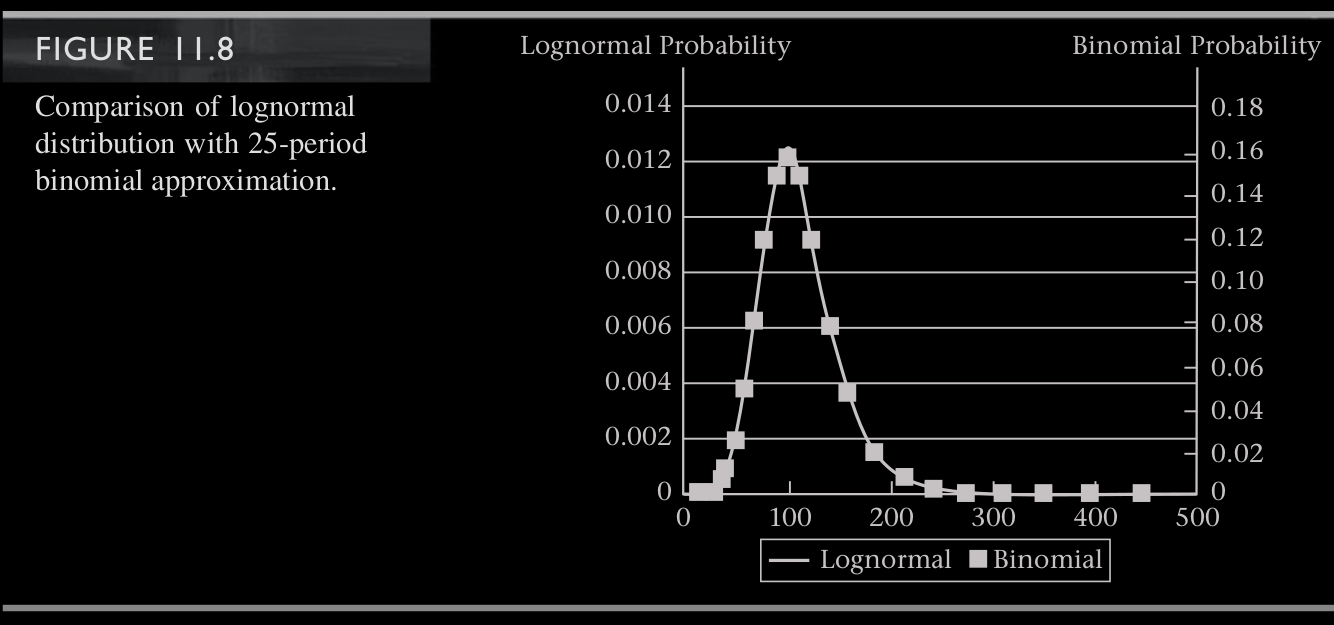
\includegraphics[scale=0.2]{figs/Figure-11-8.png}
\end{center}
\end{frame}
%-------------- end slide -------------------------------%}}}
%-------------- start slide -------------------------------%{{{ 1
\begin{frame}[fragile]
	\frametitle{Alternative Binomial trees}

	\begin{minipage}{0.3\textwidth}
		\begin{center}
		Binomial\\
		Tree

		\begin{align*}
			u & =e^{(r-\delta)h + \sigma \sqrt{h}} \\
			d & =e^{(r-\delta)h - \sigma \sqrt{h}}
		\end{align*}
		\end{center}
	\end{minipage}
	\hfill
	\begin{minipage}{0.3\textwidth}
		\begin{center}
		Cox-Ross-Rubinstein\\
		binomial tree

		\begin{align*}
			u & =e^{ + \sigma \sqrt{h}} \\
			d & =e^{ - \sigma \sqrt{h}}
		\end{align*}
		\end{center}
	\end{minipage}
	\hfill
	\begin{minipage}{0.3\textwidth}
		\begin{center}
		 Lognormal \\ tree

		\begin{align*}
			u & =e^{(r-\delta-0.5\sigma^2)h + \sigma \sqrt{h}} \\
			d & =e^{(r-\delta-0.5\sigma^2)h - \sigma \sqrt{h}}
		\end{align*}
		\end{center}
	\end{minipage}
	\pause
	\bigskip
	\mySeparateLine
	\bigskip
	\begin{itemize}
		\item Even though the values of $u$ and $d$ are deferent, the ratio, which measures volatility,
			remains the same:
			\begin{equation*}
				u/d = e^{2\sigma \sqrt{h}}.
			\end{equation*}
		\item Once $u$ and $d$ are determined, the rest computations for option price remain the same.
		\item All three methods of constructing a binomial tree yield different option prices for finite
			n, but they approach the same price as $n\to\infty$.
	\end{itemize}
\end{frame}
%-------------- end slide -------------------------------%}}}
%-------------- start slide -------------------------------%{{{ 1
\begin{frame}[fragile]
	\frametitle{Is the Binomial model realistic?}
	\begin{center}

	The binomial model is a form of the random walk model, adapted to modeling stock prices. The lognormal random walk model in this section assumes among other things, that
	\bigskip

	Volatility is constant\\[0.5em]

	``Large" stock price movements do not occur \\[0.5em]

	Returns are independent over time\\[0.5em]

	\bigskip
	\mySeparateLine
	\bigskip

	All of these assumptions appear to be violated in the data

	\end{center}
\end{frame}
%-------------- end slide -------------------------------%}}}
